\chapter{Advantages and Disadvantages of IaaS Systems}
\label{chap:advantages}

The classical approach of deploying software, which was the case before the invention of cloud computing, is called "Dedicated Hardware". Using this approach companies buy hardware on their own which is dedicated only for the intended software, which should run on it. To provide a good level of service, usually companies buy hardware which can handle worst case scenarios and load peaks \cite{Gajbhiye_2014}.

The problem of this approach is, that if the system runs on average work load, the full hardware capacities are not used and therefore there are resources which are wasted like CPU cycles, storage space or RAM. If there are peaks in the work load this can result in a huge waste of resources of in a poor service of the software, if the hardware is not designed for such high peaks. Figure \ref{fig:dedicated_hardware_utilization} shows some of these problems.

\begin{figure}[h!]
	\centering
		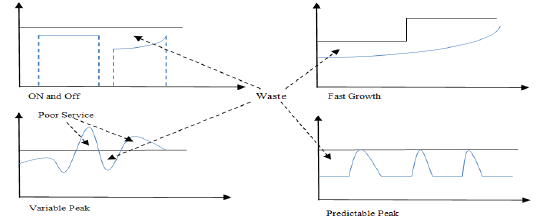
\includegraphics[width=0.75\textwidth]{dedicated_hardware_utilization}
	\caption{Dedicated Hardware Model - Utilization Waste \cite{Gajbhiye_2014}}
	\label{fig:dedicated_hardware_utilization}
\end{figure}

In cloud computing this waste of resources can be prevented by dynamically assign resources when needed. For example, if the cloud computing system identifies that there is an overload, it can just add another virtual machine which can also handle requests. Later if there is less workload this VM can be shutdown and the available resources can be used for other services. Figure \ref{fig:cloud_computing_utilization} shows the dynamic resource allocation of cloud computing.

\begin{figure}[h!]
	\centering
		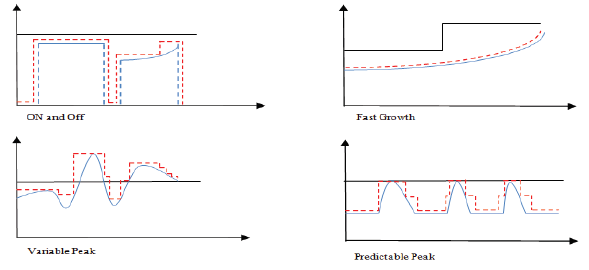
\includegraphics[width=0.75\textwidth]{cloud_computing_utilization}
	\caption{Cloud Computing Model - Dynamic Resources \cite{Gajbhiye_2014}}
	\label{fig:cloud_computing_utilization}
\end{figure}